\section{Auswertung}\raggedbottom 
\label{sec:auswertung}

\subsection{Statistische Auswertung}

\subsubsection{Erkennungsrate}
\label{sub:erkennungsrate}

Ein wichtiger Faktor, um Karten in Videos zu erkennen, ist wie verlässlich ein Verfahren die Karten erkennt. Die Ergebnisse der in \ref{sub:durchführung} besprochenen Durchführung finden sich in Tabelle \ref{table:result} wieder.

\begin{table}
\centering
	\begin{tabular}{  l c c c c  }
	  Verfahren & Normal & Rotation & Helligkeit & Rotation+Helligkeit \\
	  \midrule
	  SIFT & 299 (99.67\%) & 2861 (95.37\%) & 2990 (99.67\%) & 2845 (94.82\%) \\
	  SURF & 295 (98.33\%) & 2925 (97.50\%) & 2964 (98.80\%) & 2940 (98.00\%) \\ 
	  ORB & 298  (99.33\%) & 2930 (97.67\%) & 2952 (98.40\%) & 2925 (97.50\%) \\
	\end{tabular}

\caption{Erkannte Karten pro Verfahren und Datensatz. In Klammern ist jeweils die prozentuale Erkennungsrate angegeben.}
\label{table:result}
\end{table}

Es lässt sich sehen, dass alle Verfahren für den normalen Datensatz eine gute Erkennungrate haben.
Es fällt auf, dass bei Rotation alle Verfahren schlechtere Ergebnisse liefern. Jedoch verliert SIFT am meisten Genauigkeit. Es verliert 5.1\% im Gegensatz zu SURF (1.1\%) und ORB (1.7\%).

Die Softmaxwerte für alle richtig klassifizierten Karten sind bei allen Verfahren relativ hoch (siehe Abbildung \ref{fig:hist}). Die Mittelwerte der Softmaxwerte sind für SIFT 82.01\%, für SURF 94.69\% und für ORB 95.42\%.
Der Durchscnitt der Softmaxwerte für falsch klassifizierte Karten ist für SIFT 0.80\%, für SURF 8.31\% und für ORB 9.71\%. 


\begin{figure}
\begin{subfigure}{.5\textwidth}
  \centering
  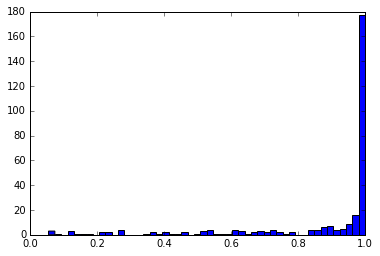
\includegraphics[width=.8\linewidth]{bilder/confidenceSift.png}
  \caption{SIFT}
  \label{fig:sfig1}
\end{subfigure}%
\begin{subfigure}{.5\textwidth}
  \centering
  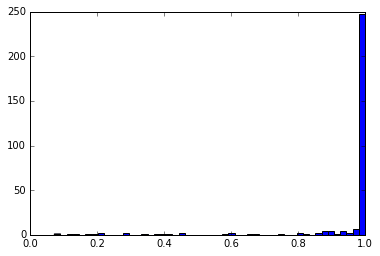
\includegraphics[width=.8\linewidth]{bilder/confidenceSurf.png}
  \caption{SURF}
  \label{fig:sfig2}
\end{subfigure}
\begin{subfigure}{.5\textwidth}
  \centering
  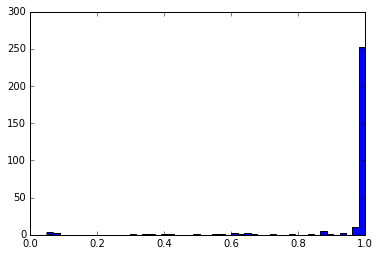
\includegraphics[width=.8\linewidth]{bilder/confidenceOrb.png}
  \caption{ORB}
  \label{fig:sfig2}
\end{subfigure}
\caption{Die Histogramme der Softmaxwerte für richtig klassifizierte Karten.}
\label{fig:hist}
\end{figure}

\subsubsection{Geschwindigkeit}

Damit ein Verfahren zur Erkennung von Karten in einem Video in Echtzeit genutzt werden kann, ist auch die Geschwindigkeit des Verfahrens relevant.
Um diese zu bestimmen, wurde die Laufzeit für die drei Verfahren gemessen. Hierbei wurde nur die Zeit gemessen, die benötigt wird, um eine Karte zu klassifizieren. Die Zeit, die benötigt wird um die Features des Trainigsdatensatzes zu berechnen, wurde nicht beachtet, da dies nur einmal gemacht werden muss, bevor die Karten klassifiziert werden.
Die Ergebnisse dieser Messung finden sich in Tabelle \ref{table:speedResult} wieder.

\begin{table}
\centering
	\begin{tabular}{  l c c   }
	  Verfahren & Zeit gesamt & Zeit pro Karte \\
	  \midrule
	  SIFT & 709s & 2.3s\\
	  SURF & 171s & 0.57s\\ 
	  ORB & 45s & 0.15s \\
	\end{tabular}

\caption{Laufzeit der einzelnen Verfahren für den Standard Datensatz in Sekunden.}
\label{table:speedResult}
\end{table}



\subsection{Bewertung der Ergebnisse}

\subsubsection{Erkennungsrate}

Die Erkennungsrate aller Verfahren ist so hoch, dass sie für den Einsatz in einem Programm zur Liveerkennung von Karten verwendet werden könnten.
Es fällt auf, dass SIFT im Gegensatz zu den anderen Verfahren am stärksten von Rotation der Karten beeinflusst ist. Dies ist erstmal überraschend, da alle Verfahren so konstruiert sind, dass die Merkmale rotationsinvariant sind.
Bei genauerer Betrachtung dieses Sachverhalts fällt auf, dass SIFT für die falsch klassfizierten rotierten Bilder viel mehr Keypoints findet, als SURF und ORB. 
Diese liegen zu einem großen Teil am Rand der Karte und nicht mehr im Bereich, wo das Kartenbild ist (siehe Abbildung \ref{fig:keypointsRot}).
Diese Keypoints und die dazugehörigen Merkmale geben keine Information über das eigentliche Aussehen der Karte.

\begin{figure}[h]
    \centering
		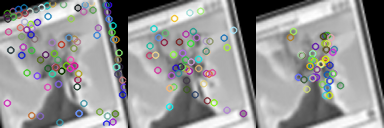
\includegraphics[scale=0.8]{bilder/keypointsRot.png}
    	\caption{Die gefundenen Keypoints sind jeweils mit farbigen Kreisen markiert. Von links nach rechts SIFT, SURF, ORB}
\label{fig:keypointsRot}
\end{figure}


Es ist insbesondere zu beobachten, das alle diese Keypoints an einer Kante liegen.
Dies lässt den Schluss zu, dass SIFT in Bildern mit kleinen Auflösungen ($128 \times 128$ Pixel), häufig Keypoints an Kanten findet, anstatt nur an Ecken.


\subsubsection{Geschwindigkeit}

In der Geschwindigkeit der Verfahren lässt sich ein klarer Unterschied erkennen. Dieser ist allerdings auch zu erwarten. SURF wurde mit dem Ziel entworfen, schneller als SIFT zu sein. Das gleiche gilt für ORB, welches in seinem Paper \footnote{\cite{Rublee:2011:OEA:2355573.2356268}} als effizientere Alternative zu SIFT und SURF vorgestellt wurde.

Damit die Klassifikation in einem Video für einen Anwender nutzbar ist, muss diese ohne große Verzögerung ausgeführt werden können. Mit 2.3 Sekunden ist SIFT eindeutig zu langsam, um zur Klassifikation genutzt zu werden. 
Auch SURF ist mit über einer halben Sekunde Verzögerung fast viermal so langsam wie ORB.
Ein großer Teil des Geschwindigkeitsvorteils von ORB lässt sich damit begründen, dass die von ORB bestimmten Merkmalsdeskriptoren binär sind. Die Berechnung der Hamming Distanz ist deutlich effizienter, als eine Berechnung der euklidischen Distanz.
